\section{Challenges \& Optimization}
\vspace{-0.5em}
In this section, we bring up some challenges and performance bottleneck we encounter that limited our speedup and how we optimized these bottlenecks. There are in total three optimization we performed.

\subsection{Redundant search space}
The first bottleneck that limits our speedup and performance is that there were a lot of redundant search state we are searching over. Our naive approach iterated over 4 orientation of each block, however, some tetromino blocks has less than 4 orientations. For example consider the I space tetromino block in Fig. \ref{fig:piece_orientation}.
\begin{figure}[h]
	\centering
	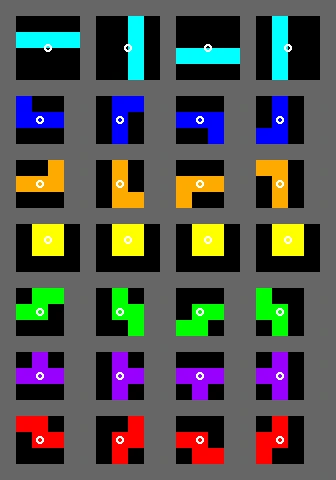
\includegraphics[width=0.2\textwidth]{SRS-pieces.png}
	\vspace{0em}
	\caption{Orientation of Tetromino Blocks. This figure shows orientation 0 to orientation 3 of all blocks from left to right}
	\label{fig:piece_orientation}
\end{figure}
It only has two unique orientations 0 and 1, the rest are just duplicate orientations. Secondly, we also assume that each block has 10 possible columm placement, which is obvious also not true since the shape of the block would limit its placement. For example, a I space block with orientation 0, would only have 6 possible column placement, otherwise the piece would go out of bound (under our game setting with column width as 10). Therefore, we were able to prune a lot of search space out, and each tetromino block has their own branching factor shown in Fig \ref{fig:tetris_table}.
\begin{figure}[h]
	\centering
	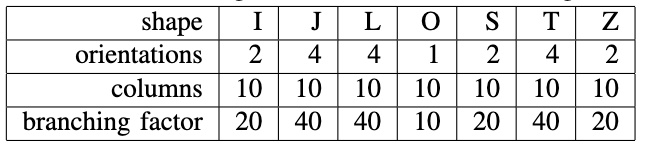
\includegraphics[width=0.5\textwidth]{tetris_table.png}
	\vspace{-1em}
	\caption{Branching Factor of Tetromino Blocks. Image reference: \ref{ref:tetrisImage}}
	\label{fig:tetris_table}
\end{figure}

% reference https://tetris.fandom.com/wiki/SRS?file=SRS-pieces.png
This optimization, however, can only be used in approach 2, otherwise it would introduce severe workload imbalance in the DFS tree, resulting in significant decrease in the speedup. In approach 2, since we are partitioning the combination space, it is easy for us to implement this but only on the orientations. We still iterate over 10 column for every blocks for coding simplicity. 

\subsection{Workload imbalance}
Here we focus on the workload imbalance of Approach 2. As mentioned previously, approach 2 can evenly partition the search space among worker threads. However, we still observed workload imbalance in the scoring phase of each worker where we take the tetris board state and output a score that indicates the wellness of the board. The imbalance is subtle but became a bottleneck when we optimized our code to a certain extent. We discovered that it was due to the function that calculates the height of each board. Since the way we find the height is checking from top to bottom of whether each row is empty and return if we found one non-empty row, this would result in a imbalance when the height of the board is different. Considering how we partitioned our search space, each threads would be responsible for a continuous range of node id thus the final board state of a thread would be similar. If one threads tends to always have a higher board state than another thread, its workload on the scoring phase would be higher resulting in a imbalance (see Fig \ref{fig:tetris_board}.) 
We solve this issue by simply storing the board height in the game object and maintaining it every time we place a tetromino on the board. This way we can get the height in constant time for any board state.
\begin{figure}[h]
	\centering
	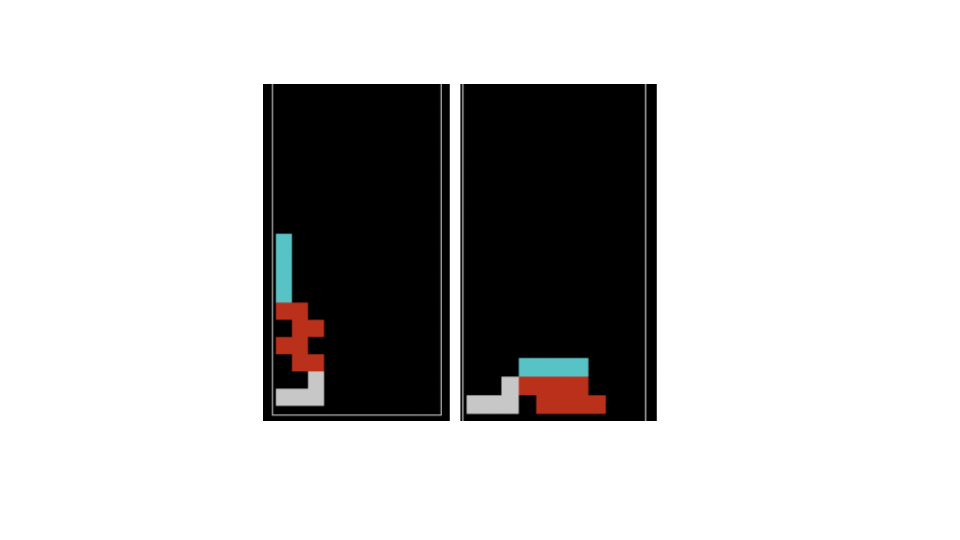
\includegraphics[width=0.5\textwidth]{tetris_board.png}
	\vspace{-3em}
	\caption{Low and High Tetris Board of Same Block Combination}
	\label{fig:tetris_board}
\end{figure}

\subsection{State caching}
Another optimization we did is that we cached the board state to avoid duplicate drops. Consider one worker thread reponsible for node 0 to node 20000. Using the formula we derived earlier we can see that consecutive nodes would have the same prefix for their tid set. For example, if node 0 corresponds to $\{ tid_{1}, tid_{2}, tid_{3},tid_{4}\}$ then node 1 would correspond to $\{ tid_{1}, tid_{2}, tid_{3},tid_{4} + 1\}$. In this case, we could cache the drop result of $\{ tid_{1}, tid_{2}, tid_{3}\}$, and reuse it. In the best case, we can save up to 40 x 3 drops, where 40 is the branching factor of the fourth block and 3 corresponds to the previous 3 drops. Currently, we are only caching depth - 1 layer of drops, more aggressive caching is possible but are harder to implement, the current implementation already can significantly lower our drop time.
